\begin{enumerate}[label=\thesection.\arabic*.,ref=\thesection.\theenumi]
\numberwithin{equation}{enumi}

\item Consider the system in Section \ref{sec:ee18btech11021}.  
\begin{align}
G(s) = \frac{1}{s(3s+1)}
\end{align}
Find the step response for the system in Fig. \ref{fig:ee18btech11027}.
%Find the settling time for the system in Fig. \ref{fig:ee18btech11027}.
%
\begin{figure}[!ht]
\begin{center}
\resizebox{\columnwidth}{!}{\tikzstyle{block} = [draw, fill=blue!20, rectangle, 
    minimum height=0.7cm, minimum width=0.7cm]
\tikzstyle{sum} = [draw, fill=blue!20, circle, node distance=1cm]
\tikzstyle{input} = [coordinate]
\tikzstyle{output} = [coordinate]
\tikzstyle{pinstyle} = [pin edge={to-,thin,black}]

\begin{tikzpicture}[auto, node distance=2.5cm,>=latex']
    % We start by placing the blocks
    \node [input, name=input] {};
    \node [sum, right of=input] (sum) {};
    \node [block, right of=sum] (controller) {G(s)};
    \node [output, right of=controller] (output) {};


    \draw [draw,->] (input) -- node {$R(s)\ +$} (sum);
    \draw [->] (sum) -- node {$E(s)$} (controller);
    \draw [->] (controller) -- node [name=y] {$Y(s)$}(output);
  \draw [->] (y) -- ++ (0,-2) -| node [pos=0.99] {$-$} (sum);
 
\end{tikzpicture}}
\end{center}
\caption{}
\label{fig:ee18btech11027_gs}
\end{figure}
%
\\
\solution The step response is
\begin{align}
Y(s) &= \frac{G(s)}{1+G(s)}\frac{1}{s}\\
&= \frac{1}{(s)(3s^2+s+1)}\\
&= \frac{-3s-1}{3s^2+s+1} + \frac{1}{s} 
\end{align}
\begin{multline}
\implies         y(t) = \lsbrak{1 - e^{-\frac{t}{6}}\lcbrak{\cos\brak{\frac{\sqrt{11}t}{6}}}}
\\
-\rsbrak{ \rcbrak{\frac{1}{\sqrt{11}}\sin\brak{\frac{\sqrt{11}t}{6}}} }u(t)
\end{multline}

\item Find the step response for the system shown in Fig. \ref{fig:ee18btech11027_gs_ds} that is  
obtained by adding the lead compensator to the system in Fig. \ref{fig:ee18btech11027_gs}
\begin{align}
D(s) = \frac{3(s+\frac{1}{3})}{(s+1)}
\end{align}
%
%the settling time for  reduces.
%
\begin{figure}[!ht]
\begin{center}
\resizebox{\columnwidth}{!}{

\tikzstyle{block} = [draw, fill=blue!20, rectangle, 
    minimum height=3em, minimum width=6em]
\tikzstyle{sum} = [draw, fill=blue!20, circle, node distance=1cm]
\tikzstyle{input} = [coordinate]
\tikzstyle{output} = [coordinate]
\tikzstyle{pinstyle} = [pin edge={to-,thin,black}]

% The block diagram code is probably more verbose than necessary
\begin{tikzpicture}[auto, node distance=2cm,>=latex']
    % We start by placing the blocks
    \node [input, name=input] {};
    \node [sum, right of=input] (sum) {};
    \node [block, right of=sum] (controller) {G(s)};
    \node [block, right of=controller,
           node distance = 4cm ] (system) {D(s)};
    % We draw an edge between the controller and system block to 
    % calculate the coordinate u. We need it to place the measurement block. 
    \draw [->] (controller) -- node[name=u] {$U(s)$} (system);
    \node [output, right of=system] (output) {};
    \coordinate [below of=u] (tmp);

    % Once the nodes are placed, connecting them is easy. 
    \draw [draw,->] (input) -- node {$R(s)\ +$} (sum);
    \draw [->] (sum) -- node {} (controller);
    \draw [->] (system) -- node [name=y] {$Y(s)$}(output);
    \draw [->] (y) |- (tmp) -| node[pos=0.99] {$-$} 
        node [near end] {} (sum);
\end{tikzpicture}

}
\end{center}
\caption{}
\label{fig:ee18btech11027_gs_ds}
\end{figure}
\solution The step response is given by 
\begin{align}
Y_{1}(s) &=\frac{G_{1}(s)}{1+G_{1}(s)}\frac{1}{s}\\
&=\frac{1}{s(s^2+s+1)}
\end{align}
%
where
\begin{align}
G_{1}(s) = G(s)D(s)=\frac{1}{s(s+1)}
\end{align}

\begin{multline}
\implies         y(t) = \lsbrak{1 - e^{\frac{-t}{2}}\lcbrak{\cos\brak{\frac{\sqrt{3}t}{2}}}}
\\
- \rsbrak{\rcbrak{\frac{1}{\sqrt{3}}\sin\brak{\frac{\sqrt{3}t}{2}}} }u(t)
\end{multline}

\item Show that the lead compensator reduces the settling time.
\\
\solution The following code generates Fig. \ref{fig:ee18btech11027} which is self-explanatory.
\begin{lstlisting}
codes/ee18btech11027.py
\end{lstlisting}

\begin{figure}[!ht]
%\begin{subfigure}{\textwidth}
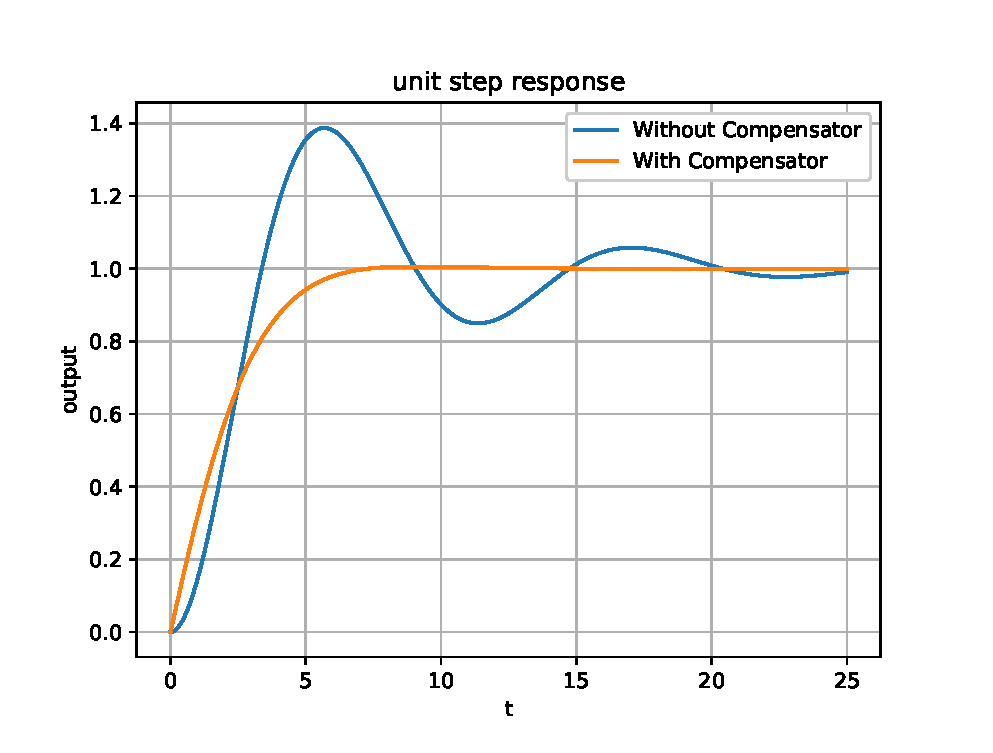
\includegraphics[width=\columnwidth]{./figs/ee18btech11027/ee18btech11027.eps} 
\caption{}
\label{fig:ee18btech11027}
\end{figure}
\end{enumerate}
